\documentclass[a4paper, 11pt, oneside]{thesis}

\usepackage[utf8]{inputenc}
\usepackage[T1]{fontenc}
\usepackage{lmodern}

\usepackage[square, numbers, comma, sort&compress]{natbib}

\usepackage{changepage}
\usepackage{float}
\usepackage[section]{placeins}

\usepackage{xcolor} 
\definecolor{rred}{HTML}{e0304e}

\lstset{
  captionpos=b,
  frame=tb,
  comment=[l]{\#},
  basicstyle=\ttfamily\footnotesize\linespread{1.2}\selectfont,
  numberstyle=\footnotesize\color{gray},
  commentstyle=\itshape,
  showstringspaces=false,
  keepspaces=true,
  aboveskip=2em,
  numbers=left,
  escapeinside={<@}{@>},
  moredelim=**[is][\color{rred}]{[@}{@]}
}

\usepackage[capitalise,noabbrev]{cleveref}
\crefname{sublstlisting}{Listing}{Listings}
\Crefname{sublstlisting}{Listing}{Listings}
\crefdefaultlabelformat{#2{\scshape #1}#3}
\AtBeginDocument{\DeclareCaptionSubType{lstlisting}}

\usepackage{varwidth}
\usepackage{verbatim}
\usepackage{stmaryrd}
\usepackage{mathtools}
\DeclarePairedDelimiter\set{\lbrace}{\rbrace}
\DeclarePairedDelimiter\bbrackets{\llbracket}{\rrbracket}
\DeclarePairedDelimiter\angles{\langle}{\rangle}
\DeclarePairedDelimiter\ttangles{\mathtt{<}}{\mathtt{>}}
\newcommand{\univ}{\ensuremath{\mathbb{U}}}

\usepackage{bussproofs}
\def\labelSpacing{1em}
\usepackage[altpo,epsilon]{backnaur}
\newcommand{\bnfmor}[1]{\bnfmore{\hspace{-1.5em}\ooalign{|\cr\hspace{1.5em}}#1}}

\usepackage{tipa}
\newcommand{\ipa}[1]{{\usefont{T3}{cmr}{m}{n}\selectfont#1}}

\usepackage{tikz}
\usetikzlibrary{chains,shapes,arrows,calc,positioning}
\tikzstyle{arrow} = [draw, -latex']
\tikzstyle{box} = [rectangle, draw=black!50, align=left, font={\ttfamily}]
\tikzstyle{init} = [circle, draw=black!50]
\tikzstyle{circ} = [circle, font={\ttfamily}]

\usepackage{siunitx}
\usepackage{csvsimple}
\usepackage{pgfplots}
\pgfplotsset{compat=1.18}
\usepackage{pgfplotstable}
\usepackage{xstring}
\pgfplotsset{where/.style 2 args={
    x filter/.code={
      \IfStrEq{\thisrow{#1}}{#2}{}{\def\pgfmathresult{}}
    }
  }
}

\graphicspath{{figures/}}
\def\datapath{data}

\begin{document}

\frontmatter

%TC:ignore
\university{{The University of Melbourne}}
\UNIVERSITY{{THE UNIVERSITY OF MELBOURNE}}
\department{{Department of Mathematics \& Statistics}}
\school{{Melbourne School of Mathematics}}
\degree{{Master of Mathematics}}
\title{{Range Thresholding on Streams}}
\shortauthors{{Sean Conlon}}
\authors{
  \texorpdfstring{\href{mailto:sconlon@student.unimelb.edu.au}{\shortauthornames}}{\shortauthornames}\\
  \small Student Number: TBA
}
\supervisor{{Dr.~Junhao Gan, Dr.~William Umboh}}
\addresses{\deptname\\\univname}
\date{October 2024}
\subject{}
\keywords{}
%TC:endignore

%TC:envir lstlisting [option:text] xall
%TC:ignore
\wordcount{\input{|"bash ./scripts/fmt-texcount.sh \jobname.tex"}}
%TC:endignore

\maketitle

\setstretch{1.3}

\fancyhead{}
\rhead{\thepage}
\lhead{}

\pagestyle{fancy}

%TC:ignore

\abstract{
  In this thesis we study an applied Computational Geometry problem known as \textit{Range Thresholding on Streams} (RTS). We review the state-of-the-art algorithm for the RTS problem, and present the details in a manner that is accessible to a wider audience, as well as providing proofs for claims omitted from the original paper \cite{GAN16}. In addition to reviewing the existing literature, we make our own contributions. First, we motivate and introduce a more-general problem which we call \textit{Dynamic Range Thresholding on Streams} (DRTS), and mathematically characterise when existing RTS algorithms can also solve DRTS. Next, we introduce and analyse a novel approximation algorithm for the DRTS problem. Finally, we demonstrate that our proposed algorithms have not only strong theoretical guarantees, but also perform well in practice via an experimental study.
}

\clearpage

\acknowledgements{
  Lorem ipsum dolor sit amet, consectetur adipiscing elit. Integer in libero posuere, sollicitudin felis vel, ultrices orci. Donec faucibus malesuada sollicitudin. Aenean vitae fermentum nisl, tincidunt faucibus tellus. Vivamus in vulputate eros, non suscipit diam. Proin eget elementum turpis. Suspendisse diam sem, rhoncus id odio ut, auctor ultrices libero. Aenean a tellus ac odio vestibulum vulputate. Maecenas venenatis neque quis urna auctor fringilla. Aliquam et augue et turpis varius auctor. Mauris ut pulvinar diam. Mauris nec imperdiet nisl.

    Vestibulum risus quam, eleifend at gravida a, sodales vel turpis. Vestibulum ante ipsum primis in faucibus orci luctus et ultrices posuere cubilia curae; Sed ipsum lacus, cursus sit amet pharetra id, interdum et erat. Vestibulum ex dui, faucibus sit amet urna dapibus, laoreet luctus dui. Nulla sem ligula, aliquet id arcu in, vestibulum egestas leo. Ut in ex elementum, commodo ipsum a, efficitur neque. Aenean rhoncus nisl vestibulum vulputate porttitor. Sed id iaculis erat, vitae aliquam quam. Vivamus vel congue diam, quis pellentesque purus. Pellentesque auctor pharetra convallis.
    
    Curabitur interdum, nisi sed tempor posuere, lorem nulla porta metus, at imperdiet lacus erat eget dui. Donec sagittis hendrerit ligula, quis laoreet leo. Donec et efficitur risus, eu pellentesque orci. Sed lobortis est eget convallis laoreet. Cras aliquam vulputate sem, ac dictum velit lacinia nec. Nunc viverra ligula ipsum, vitae fermentum risus imperdiet vel. Suspendisse sit amet sodales mi, ac malesuada ipsum. Aenean commodo quam sed leo euismod laoreet. Aliquam scelerisque nisl quis risus fermentum aliquam. Aenean faucibus mi et imperdiet interdum. Nunc vestibulum convallis accumsan. Phasellus quis dolor eget quam porta pulvinar. Sed ullamcorper justo vel elit aliquam, id suscipit augue convallis. Donec vehicula iaculis interdum.
}

\clearpage


\tableofcontents
% \listoffigures
% \listoftables
% \lstlistoflistings
%TC:endignore

\addtocontents{toc}{\vspace{1em}}

\mainmatter	
\pagestyle{fancy}
\setstretch{1.5}

\clearpage

\def\chaptertitle{Introduction}

\lhead{\emph{\chaptertitle}}

\chapter{\chaptertitle}
\label{ch:introduction}

This thesis studies an applied problem from Computational Geometry called \textit{Range Thresholding on Streams} \cite{GAN16}. The problem is best motivated through an example related to trading in the share market. Suppose that we are a high-stakes trader, and we pay close attention to the trading volumes in sensitive price ranges. For example, we may know that substantial limit orders in certain price ranges may indicate significant price downfall. We therefore wish to receive timely alerts for queries of the form: 

\textit{"Alert me when \text{100,000} shares of AAPL (Apple Inc.) have been sold in the price range \text{[200, 205]} from now."}

More formally, the Range Threshold on Streams (RTS) problem can be formulated as follows. Consider an unbounded stream of elements $\{e_i\}^{n}_{i=1}$ where each element $e_i$ contains a \textit{value} $v(e_i) \in \mathbb{R}$ and a \textit{weight} $w(e_i) \in \mathbb{Z}$. An RTS query $q$ comprises of a tuple $(R_q, \tau_q)$ where $R_q = [x,y]$ is a subset of the real line, and $\tau_q \in\mathbb{N}$ is some \textit{threshold}. Let $S(q)$ be the set of stream elements $e_i$ such that 
\begin{itemize}
    \item $e_i$ is received after the time $q$ is registered and,
    \item has value $v(e)$ falling into $R_q$. 
\end{itemize}
The query \textit{matures} the instant that $\sum_{e\in S(q)}w(e)\geq \tau_q$. The Range Thresholding on Streams problem is to design an algorithm or data structure that can efficiently support and process a huge number of simultaneous RTS queries  in terms of both space and computational cost. 

As described in the RTS literature \cite{GAN16, DBLP:conf/sigmod/ZhangGBKCZ22}, an RTS query $q$ intuitively detects when the interval $R_q$ becomes a \textit{hot spot}, and solutions to the RTS problem are required for applications which involve rapid responses to such hot spots, such as the as our earlier example in stock trading.

The RTS problem is deceptively simple at first glance - one can easily solve the problem with the following polynomial-time algorithm; whenever a stream element $e$ arrives, one checks if $e\in R_q$ for each registered query $q$, and update some counter $c_q$ if so. The instant that $c_q \geq \tau_q$ report maturity for the query. For a set of $m$ queries the cost of processing a $n$ streams becomes a prohibitively large $O(nm)$ - suggesting that the naive algorithm becomes computationally intractable when attempting to support a large number of queries. 

Despite the number of applications for the RTS problem \cite{DBLP:conf/sigmod/ZhangGBKCZ22}, it was only until recently that the first algorithm was proposed that escapes the $O(nm)$ barrier of the naive algorithm \cite{GAN16}. 

\section{Motivation}
\label{sec:motivation}
This thesis is primarily motivated to extend the literature to define and solve a more general version of the RTS problem, in which the interval of interest for a given query $R_q$, is allowed to become \textit{dynamic}. 

Returning to our example related to the Stock market, Traders will often be interested in buy/sell orders being placed within ranges related to the so-called \textit{volume weighted average price} (VWAP) \cite{vwap}. Recall that the formula for VWAP is given by 
\begin{equation}
    \frac{\sum_{e}v(e) \times w(e)}{\sum_{e}w(e)}
\end{equation}
where $v(e)$ denotes the \textit{price} or \textit{value} of order $e$ and $w(e)$ denotes the corresponding \textit{volume} or \textit{weight}. If a trader were to register an alert of such as:

\textit{"Notify me when $\tau$ shares of limit orders have been registered within $x$\% of VWAP"}

There is currently no algorithm to do so, as existing RTS solutions require that the interval of interest for a given query $R_q$ remains fixed over the lifetime of said query, whereas endpoints determined by percentages of VWAP will \textit{evolve} with new trades as in $(1)$. 

Our goal therefore, is to mathematically formalise this more general type of query, where the endpoints or region of interest $R_q$ is allowed to \textit{change} with the introduction of each new stream element. Similar to the RTS problem, we then want to design salable solutions to manage a large number of simultaneous queries. 

\section{Thesis Outline}
\label{sec:doc-outline}

The remainder of the thesis is outlined as follows; in \cref{ch:preliminaries} we cover all the necessary mathematical material to understand and analyse the state of the art solutions to the RTS problem. In \cref{ch:rts} we formally define the RTS problem, and briefly cover some existing solutions to RTS. The bulk of the chapter is then devoted to describing the state of the art \textit{DT Algorithm} for the RTS problem, and formally proving it's correctness and sub-quadratic run time. In \cref{ch:drts} we formalise an extension of the problem, which we call \textit{Dynamic Range Thresholding on Streams} (DRTS), as described in \cref{sec:motivation}. For the remainder of the chapter, we demonstrate how the DT Algorithm can be extended to solve the dynamic version of the problem, as well as propose a novel algorithm, in which we trade accuracy for speed to solve a special class of DRTS instances. Finally, we demonstrate that our algorithms not only have strong theoretical properties, but also perform well in practice via an experimental evaluation on synthetic and real data. 

\clearpage

\def\chaptertitle{Preliminaries}

\lhead{\emph{\chaptertitle}}

\chapter{\chaptertitle}
\label{ch:preliminaries}

\section{Analysis of Algorithms}
\label{sec:anaylsis-of-algorithms}

With Algorithms and Data Structures being a core topic of this thesis, we require the formal mathematical language that is used to describe and evaluate their performance. In addition, we also need to specify a so-called model of computation, which defines the set of \textit{operations} a computer has available to formulate an algorithm.

\subsection{Word-RAM Model \& Big Oh Notation}
In this thesis, we consider so-called the Word-RAM model \cite{DBLP:conf/stoc/FredmanW90} which models as computer as having a contiguous array of \textit{Memory} registers and a \textit{CPU} which can perform: 
\begin{itemize}
    \item \textbf{Regiser (Re-)Initialization}: Set the content of a register in memory to a fixed value, or to the content of another register.
    \item \textbf{Arithmetic Operations}: Take two integers $a$ and $b$ stored in two registers, calculate the following and then store the result in a register.
    \item \textbf{Comparison and Branching}: Compare two integers $a$ and $b$ stored in two registers and decide which of the following is true: $a<b, a=b$ and $a>b$.
    \item \textbf{Memory Access}: Take the memory address $p$ stored in a register, then perform one of a read or write operation at address $p$.
\end{itemize}

Every algorithm can be viewed as a sequence of these four atomic operations. The \textit{running time cost} of an algorithm is the measured by the number of operations in the sequence, as a function of the size of the input $n$. The \textit{space consumption} of an algorithm is the measured by the footprint of memory cells which it touches, that is, the peak memory usage when the algorithm is running. We will commonly describe the growth of said function in terms of their Big-$O$, Big-$\Omega$ and Big-$\Theta$ complexity defined as follows

\begin{definition}[Big-$O$ Notation]
    We say $f(n)$ grows asymptotically no faster than $g(n)$ if there exists two positive constants $c_1$ and $c_2$ such that $f(n)\leq c_1 g(n)$ for all $n\geq c_2$. We define $O(g(n))$ as the family of functions that grow asymptotically no faster than $g(n)$.
\end{definition}

\begin{definition}[Big-$\Omega$ Notation]
    We say $f(n)$ grows asymptotically no slower than $g(n)$ if there exists two positive constants $c_1$ and $c_2$ such that $f(n)\geq c_1 g(n)$ for all $n\geq c_2$. We define $\Omega(g(n))$ as the family of functions that grow asymptotically no slower than $g(n)$.
\end{definition}

\begin{definition}[Big-$\Theta$ Notation] $\Theta(g(n))$ is the family of all functions of $n$ that grow \textit{asymptotically as fast as $g(n)$}. That this $\Theta(g(n)) = O(g(n))\bigcap\Omega(g(n))$.
\end{definition}

We will describe the \textit{time complexity} of an algorithm as the measurement of its running cost of via such notations. Analogously, we define the same for the \textit{space complexity} of an algorithm as a measure of its space consumption. 

\subsection{Amortised Analysis}
\label{ssec:amortised-analysis}

The commonly used big-$O$ can sometimes lead to an overly pessimistic indication of an algorithms performance. \textit{Amortised Analysis} introduced by Tarjan \cite{doi:10.1137/0606031} addresses this by instead considering the computational cost or runtime averaged across a sequence of atomic operations $\sigma_1, \sigma_2, \dots, \sigma_n$. 

Where amortised analysis is particularly useful (and also where it will be applied in this thesis), is to demonstrate that the run time of expensive but infrequent operations can be \textit{averaged} across a sequence of common, inexpensive ones. There are two methods for demonstrating the amortised runtime of a data structure, though in this thesis we will only consider the so-called \textit{Accounting Argument.} 

Also sometimes referred to as a \textit{prepaid argument}, suppose $cost(\sigma_i)$ denote the true cost of an operation $\sigma_i$. The goal of the accounting argument is to assign \textit{amortised costs} $a(\sigma_i)$ such that for any sufficiently long sequence of operations
$$\sum_{i=1}^{n}cost(\sigma_i)\leq\sum_{i=1}^{n}a(\sigma_i)$$


\section{Binary Heap Data Structures}
\label{sec:heap-data-structs}

The Binary Heap, or as we will simply refer to as a \textit{Heap}, is a data structure which is commonly visualised as a nearly-complete binary tree; in which each level of the tree, except for possibly the last, is completely filled. The lowest level of the tree, is filled from left to right. Each node $i$ in the heap contains up to three pointers, one to the Parent$(i)$, and the remaining two pointers possible to the left or right child of i which we denote by Right$(i)$ and Left$(i)$.

In practice, heaps are commonly implemented as array-like structures $A[1:n]$ that support a \texttt{HeapSize()} method to return the number of elements present in the heap. Under an array representation there is a simple $O(1)$ procedure to find the left, right and parent of a given heap element based on its index $i = 1,\dots,\texttt{HeapSize()}$: 
\begin{algorithm}
\begin{algorithmic}[1]
\Procedure{Parent}{$i$}
\State \textbf{return} $\lfloor i/2\rfloor$
\EndProcedure
\end{algorithmic}
\end{algorithm}


\begin{algorithm}
\begin{algorithmic}[1]
\Procedure{Left}{$i$}
\State \textbf{return} $2i$
\EndProcedure
\end{algorithmic}
\end{algorithm}

\begin{algorithm}
\begin{algorithmic}[1]
\Procedure{Right}{$i$}
\State \textbf{return} $2i+1$
\EndProcedure
\end{algorithmic}
\end{algorithm}

In this thesis we will often leverage a particular type of heap known as a \textit{min-heap}. In a min-heap, the elements of the data structure are organised such that for every node/index $i$, other than the root:
\begin{equation}
    \text{Parent}(i).\text{value} \leq i.\text{value} \equiv A[\text{Parent}(i)] \leq A[i]
\end{equation}
where equation $(2.1)$ is called the \textit{min-heap property}. Our motivation for studying heaps in this thesis is to take advantage of the min-heap property to create an efficient priority queue data structure. To this end, we will often make use of the following lemma

\begin{lemma}
    Given a Min-Heap on n elements, the minimum element can be found in $O(1)$ time.
\end{lemma}
\begin{proof}
    By the min-heap property in $(2.1)$ we are guaranteed that the root (or equivalently $A[1]$ in an array-like implementation) is the smallest element, which can be accessed in constant time.
\end{proof}

\subsection{Heapify}
\label{ssec:heapify}

Given an array $A[1:n]$ we require an efficient procedure to reorganise the elements of the array such that the Min-Heap property 2.1 is satisfied. This procedure of transforming an existing array into a heap is referred to as \textit{heapifying} and can be performed surprisingly fast. Consider the following procedure as described in \textit{Cormen et. al} \cite{cormen01introduction}:

\begin{algorithm}
\caption{Build Min-Heap}\label{alg:heapify}
\begin{algorithmic}[1]
\Procedure{Heapify}{$A[1:n]$}
\For{$i = \lfloor n/2 \rfloor \dots 1$}
\State \text{Min-Heapify}($A[1:n], i)$
\EndFor
\EndProcedure
\State
\State
\Procedure{Min-Heapify}{$A[1:n]$, i}
\State $l\gets \text{Left}(i)$
\State $r\gets \text{Right}(i)$
\If{$l\leq A.\text{HeapSize() and} A[l] < A[i]$}
\State \text{smallest} $\gets i$
\EndIf
\If{$r\leq A.\text{HeapSize() and} A[r] < A[\text{smallest}]$}
\State \text{smallest} $\gets r$
\EndIf
\If{\text{smallest}$\neq i$}
\State\text{swap $A[i]$ with smallest}
\State\text{Min-Heapify($A[1:n]$, smallest)}
\Comment{recursive call}
\EndIf
\EndProcedure



\end{algorithmic}
\end{algorithm}



\section{Logarithmic Rebuilding}
\label{sec:logarithmic-rebuilding}

\textit{Logarithmic Rebuilding}, also known as the \textit{Logarithmic Method} is a general technique proposed by Bentley and Sax \cite{BENTLEY1980301} for transforming a \textit{static} data structure, which does not support insertions or deletions into a data structure which is \textit{partially dynamic}; that is, supports insertions but not necessarily deletions.

The logarithmic method can be applied to so-called \textit{decomposable problems}. Consider a set of input elements $S$ which can be partitioned into disjoint subsets $S_1$ and $S_2$. A query on $S$ is \textit{decomposable} if the result of the query can be detetmined in constant time given the result of the query on $S_1$ and $S_2$. For a simple illustration of a decomposable query, consider the query $x\in S$ - the result of which can be immediately determined from $x\in S_1$ and $x\in S_2$. Given a data structure that supports a decomposable query, we now describe how to apply the logarithmic method to make the data structure partially dynamic. 

Let $S$ be the number of elements that have been inserted so far into the data structure (initially $S=\emptyset$). At all times, the method partitions $S$ into $h = \lfloor\log n \rfloor+1$ pairwise disjoint partitions $S_0, \dots, S_{h-1}$ where $n = |S|$. At all times over the life of the data structure, $S_i$ is either empty, or contains exactly $2^i$ elements. Associated to each $S_i$ is a copy of the static data structure $T_i$ on the possible $2^i$ elements of $S_i$.

\subsection{Insertion}
\label{ssec:logarithmic-rebuilding-insertion}

Consider a new element $e$ being added to $S$. We first determine the smallest $i$ such that $S_i = \emptyset$. In the case that $i=0$ we are done, otherwise $i>0$ and we untion $S_0,\dots,S_{i-1}$ along with $e$ into $S_i$. Note that this results in 
\begin{align*}
    |S_i| &= 2^0 + \dots + 2^{i-1} + 1 \\
          &= 2^i
\end{align*}
We now reset $S_j \leftarrow \emptyset$  and destroy the associated data structures $T_j$ for $j=0,\dots i-1$. Notice that this
method is general as it never \textit{modified} the data structure to introduce a method for insertion, but rather performed a systematic rebuild of the structure.

\subsection{Query}
\label{ssec:logarithmic-rebuilding-query}

The necessity for decomposable queries now becomes obvious. To perform a query $q$ on $S$, we run $q$ through $S_0, \dots, S_{h-1}$ and then use the results to answer the query for $S$.

\subsection{Analysis}
\label{ssec:logarithmic-rebuilding-analysis}

We now ask, what running time overheads does this method add to the running time of the algorithms that comprise our underlying data structure. Suppose for an input instance of size $n = |S|$ our static data structure can be build in time $build(n)$, answer queries in $query(n)$ and occupies space at most $space(n)$. We have the following theorem.

\begin{theorem} The semi-dynamic structure that results from logarithmic rebuilding uses at most $O(\sum_{i=0}^{h-1}space(2^i))$ space, answers a query in $O(\sum_{i=0}^{h-1}query(2^i))$ time and supports insertions in at most $O(\sum_{i=0}^{h-1}2^{-i}build(2^i))$ amortised time.
\end{theorem}

\begin{proof}
    We shall prove each claim of the theorem separately. 

    \textbf{Space}: Since $S_0,\dots,S_{h-1}$ forms a partition of $S$, it follows that the space of the total structure $T$ is equal to 
    \begin{align*}
        space(T) &= \sum_{i=0}^{h-1}space(S_i) \\
               &\leq \sum_{i=0}^{h-1}space(2^i)
    \end{align*}

    \textbf{Query:}  A query on $S$ now involves a query on $S_0, \dots, S_{h-1}$ plus some constant overhead. Similar to our analysis of the space complexity this is given by 
    $$query(S)\leq \sum_{i=0}^{h-1}query(2^i)$$

    \textbf{Insertion:} It is clear that some insertions are cheaper then others, for example when $i=0$, we can insert in $O(1)$, though in the worst case, an insertion can result a recombination over the $h = O(\log n)$ partitions. Given this worst-case scenario occurs relatively infrequently, we will instead analyse the \textit{amortised} time complexity, as described in \cref{ssec:amortised-analysis}, of an insertion via the following argument. 

    Recall that to insert an element we destroy the data structures on $S_0,\dots, S_{i-1}$ and then build on the $2^i$ elements in $S_i$. Thus the build time is precisely $build(2^i)$. We charge the cost over the $2^i$ elements and thus each element bears $build(2^i) / 2^i$ cost. After performing $n$ insertions, we ask how much cost can be charged this way?  We make the observation that, an element can only move from a lower indexed subset $S_i$ to a higher one, $S_j$ where $i < j$. Hence an element can be amortised at most once over every group $i = 0,\dots h-1$, bringing its amortised cost to  
    $$O\left(\sum_{i=0}^{h-1}\frac{1}{2^i}build(2^i)\right)$$
\end{proof}


\section{Distributed Tracking}
\label{sec:dist-tracking}

We make a brief excursion to the field of \textit{Distributed Computing} to consider a seemingly unrelated problem known as \textit{Distributed Tracking}. Also known as \textit{Distributed Monitoring} or \textit{Distributed Functional Monitoring} it models the following scenario: Consider a coordinator $q$ and a set of participants $S_1, \dots, S_h$. Each participant has a corresponding counter $c_i$, each initialised to 0, and the coordinator has some \textit{tolerance} $\tau \in \mathbb{N}$. At each time step, at most one of the counters are incremented; that is, one or zero counters increase. The goal of the distributed tracking problem is to design an \textit{efficient} algorithm for the coordinator to report the instant that 
$$\sum_{i=1}^{h}c_i = \tau$$
It is assumed that the coordinator and participants have a two-way communication channel, so that a participant may report its counter $c_i$ upon request from the coordinator, or at any time it pleases. By the term \textit{efficient}, we mean to design an algorithm that \textit{minimises} these total number of \textit{messages} between the coordinator and participant.


\begin{figure}
\begin{center}
\begin{tikzpicture}[scale=0.15]
\tikzstyle{every node}+=[inner sep=0pt]
\draw [black] (37.7,-20.7) circle (3);
\draw (37.7,-20.7) node {$q$};
\draw [black] (37.7,-20.7) circle (2.4);
\draw [black] (24,-38.2) circle (3);
\draw (24,-38.2) node {$S_1$};
\draw [black] (52.3,-38.2) circle (3);
\draw (52.3,-38.2) node {$S_3$};
\draw [black] (37.7,-38.2) circle (3);
\draw (37.7,-38.2) node {$S_2$};
\draw [black] (25.5,-35.7) -- (35.81,-23.03);
\fill [black] (35.81,-23.03) -- (34.91,-23.33) -- (35.69,-23.96);
\draw [black] (37.7,-35.2) -- (37.7,-23.7);
\fill [black] (37.7,-23.7) -- (37.2,-24.5) -- (38.2,-24.5);
\draw [black] (50.8,-35.3) -- (39.7,-22.93);
\fill [black] (39.7,-22.93) -- (39.87,-23.86) -- (40.61,-23.19);
\end{tikzpicture}
\caption{An example of a Distributed Tracking instance on $h=3$ participants.}
\end{center}
\end{figure}


For illustrative purposes consider the following naive algorithm for the distributed tracking problem, where at each time step if a participants counter $c_i$ has been incremented, the corresponding participant $s_i$ reports it's new count to the coorindator. This clearly results in $O(\tau)$ messages over the course of the algorithm.

A more efficient algorithm, which we will make frequent use of in this thesis, is a result of Cormode \cite{Cormode2011}, though is presented (along with its proof) in a much more simplified manner.  
\begin{algorithm}
\caption{Efficient Distributed Tracking}\label{alg:dist-tracking}
\begin{algorithmic}[1]
\Procedure{DistributedTracking}{threshold $\tau$, participant set $S_1,\dots,S_h$}
\If{$\tau\leq6h$}
    \State \text{Commence brute-force algorithm by sending $O(\tau) = O(h)$ messages}
\EndIf
\State \text{Assign to each participant \textit{slack}} $\lambda \leftarrow \lfloor \tau/2h\rfloor$
\State \text{Assign to each participant $\bar{c}_i$ the value of $c_i$ the last time a signal was sent to $q$}
\For{\text{each timestamp}}
\If{$c_i - \bar{c}_i = \lambda$}
\State \text{participant $S_i$ transmits a signal to $q$}
\State $\bar{c}_i \gets c_i$
\EndIf
\State \text{after $q$ collects $h$ notifications break and set } $\tau^\prime\leftarrow\tau-\sum_{i=1}^{h}c_i$
\EndFor
\State \textbf{return} \text{DistributedTracking}$(\tau^\prime, S_1,\dots,S_h)$ \Comment{recursive call}
\EndProcedure
\end{algorithmic}
\end{algorithm}

\begin{theorem}[Correctness and Complexity]  For a participant set $S_1,\dots, S_h$ and threshold $\tau$ \cref{alg:dist-tracking} correctly reports the instant that $\sum_{i=1}^{h}c_i = \tau$. Moreover, the algorithm requires $O(h\log\tau)$ messages.
\end{theorem}
\begin{proof}
We begin by showing correctness. In the case that $\tau\leq6h$ correctness is trivial from using the brute force algorithm. To show correctness, we therefore must show that $\tau^\prime$ in line 12 is never negative. Observe that a transmission is sent every $\lambda$ counter increases, so 
\begin{align*}
    \sum_{i=1}^{h}c_i \leq h\lambda &= h \left\lfloor\frac{\tau}{2h} \right\rfloor \\
    &\leq \tau/2
\end{align*}
Thus in line 12 we have $\tau^\prime = \tau - \sum_{i=1}^{h}c_i\geq\tau/2 \geq 0$ concluding that the algorithm correctly reports maturation.

To analyse the efficiency of the algorithm, it is clear from lines 2 and 12 that each call to the procedure necessitates $\Omega(h)$ messages. We now bound the number of recursive calls which can be made via line 14. Let $T_h(\tau)$ denote the total messages sent for an instance of threshold $\tau$ and $h$ participants, our earlier analysis shows that at each recursive call, the threshold is reduced by a factor of at most $1/2$, leading to the recurrence relation
$$T_h(\tau) = T_h\left(\frac{\tau}{2}\right) + O(h)$$
It is rudimentary to show that this leads to a total of $O(\log\tau)$ recursive calls. Combined with the $\Omega(h)$ messages per call - this leads to a total of $O(h\log\tau)$ messages throughout the algorithm.
\end{proof}

\clearpage

\def\chaptertitle{Range Thresholding on Streams}

\lhead{\emph{\chaptertitle}}

\chapter{\chaptertitle}
\label{ch:rts}

\section{Problem Definition}
\label{sec:rts-definition}
We will now formally define the Range Threshold on Streams (RTS) problem. Given a constant integer $d\geq 1$, we consider the \textit{data space} $\mathbb{R}^d$. The \textit{data stream} is an unbounded sequence of elements where the $i$-th $(i\geq1)$ element is denoted as $e_i$ and is said to arrive a time $i$. Each element $e_i$ carries two static fields; $v(e_i)$ - a point in the data space and a weight $w(e_i)\in\mathbb{Z}$. An \textit{RTS query} $q$ specifies a $d$-dimensional axis-parallel rectangle $R_q$ and a given integer threshold $\tau_q$.

If the query is issued after receiving $e_j$ for some $j\geq 1$ then for $t\geq j+1$ we define $S(q,t)$ to represent the elements $e_{j+1},e_{j+2},\dots,e_t$ that \textit{stab} $R_q$. That is, 
$$S(q, t) := \{e_i | j < i \leq t \text{ and } e_i \in R_q\}$$
Define
$$W(q, t) := \sum_{e\in S(q,t)}w(e)$$
Then the \textit{maturity time} of a query $q$ is the smallest $t$ such that $W(q,t)\geq \tau_q$. For a steam of length $n$ (that is, the length of the stream at this point) we will abbrevaiate $S(q,n)$ as $S(q)$ and $W(q, n)$ as $W(q)$.

The RTS problem is to simultaneously support a set of $m$ RTS queries and to correctly report the maturity time of a each query. In addition to supporting a given set of RTS queries, a solution must also support the following two operations, Register$(q)$: accept a new query at the current moment (after the arrival of $e_n$) and Terminate$(q)$: stop a given query $q$.

\section{Benchmark Solutions}
\label{sec:benchmark-solutions}

The RTS problem is deceptively simple at first glance, given a new stream element $e$ we can check for each query $q$ whether $e \in R_q$ and then increment $W(q)$ accordingly. This algorithm is trivially correct, though results in a quadratic $\Theta(nm)$ computation. Whilst a quadratic runtime appears innocent, this method becomes intractable when $m$ is large. Our goal therefore, is to aim for subquadratic runtime.

We also emphasis that we are considering an \textit{unboundedly} long stream of elements, all solutions explored are restricted to have a memory footprint in terms of $m$, as a Data Structure on the data stream itself is guarnateed to become prohibitively large.

\subsection{Naive Algorithm}
\label{sec:naive-algorithm}

As a simple baseline approach we will formally outline the most naive algorithm for solving the RTS problem

\begin{algorithm}
\caption{Naive RTS}\label{alg:naive-rts}
\begin{algorithmic}[1]
\Procedure{Naive-RTS}{query set $Q^*$}
\State \text{for each $q\in Q^*$ initialise $c_q\gets 0$}
\For{ \text{each stream element $e$}}
\For{ \text{each $q\in Q^*$}}
\State \text{if $e\in R_q$ set $c_q \gets c_q + w(e)$}
\State \text{if $c_q \geq \tau_q$, mature query $q$}
\EndFor
\EndFor
\EndProcedure
\end{algorithmic}
\end{algorithm}

\subsection{Stabbing Data Structures}
\label{sec:stabbing-data-structs}

A well-studied type of query in the Computer Science literature is the so-called stabbing query

\begin{definition}[Stabbing Query] Given a point $v$ in the data space $\mathbb{R}^d$ report the set of intervals $I$ in some set $Q$ such that $v \in I$. The returned set of queries are set to \textit{stabbed} by $Q$.
\end{definition}

There are a number of data structures \cite{DBLP:conf/soda/Rahul15} that support Stabbing queries, which can naturally be applied in the context of the RTS problem. We consider some notable examples below. 

\textbf{Interval Trees.}

\textbf{R Trees.}

\section{DT Algorithm}
\label{sec:DT-algorithm}

As we have seen, all benchmark solutions are unable to escape the quadratic trap in runtime which become impractical for massive values in $m$ and $n$. In this section, we present the state of the art \textit{DT Algorithm} \cite{GAN16}, as well as prove its correctness and sub-quadratic runtime.

\subsection{Constrained RTS Case}
\label{ssec:constrained-DT-algorithm}

For the moment, we restrain the RTS problem in the following ways: Set the dimension of the data space $d = 1$ and assume for each stream element we have $w(e) =1$. Moreover, we enforce that all queries are registered at the beginning, before receiving the first stream element, and no query is allowed to be registered afterwards. We refer to this latter condition as the \textit{one-time registration constraint}.

We will now present and analyse a version of the DT Algorithm for solving this constrained problem, before extending the algorithm to solve the most general version of RTS problem given in \cref{sec:rts-definition}.

\textbf{The Endpoint Tree.} We begin by denoting $Q^*$ as the set of registered RTS queries. The first step of the algorithm is to construct a special binary tree $\mathcal{T}$ on the sorted endpoints of the intervals in $Q^*$. For the remainder of this thesis, any tree constructed this way will be reffered to as an \textit{endpoint tree}. For each vertex $v\in V(\mathcal{T})$ we define its \textit{jurisdiction interval} as follows: 

\begin{definition}[Jurisdiction Interval]
    For each $v\in V(\mathcal{T})$ the \textit{jurisdiction interval associated with v}, denoted by $I(v)$. When $v$ is a \textit{leaf node} of $\mathcal{T}$ then $I(v) := [x, x^\prime)$ where $x$ is the endpoint associated with $v$ and $x^\prime$ is the endpoint associated with the leaf succeeding $v$. In the case that $v$ is the rightmost leaf of $\mathcal{T}$ define $x^\prime = +\infty$. When $V$ is not a leaf, define $I(v) := I(v.left) \cup I(v.right)$ where \textit{v.left} and \textit{v.right} denote the left and right child nodes of $v$.
\end{definition} 

In addition to each vertex $v$ having a jurisdiction interval, we also initialise a \textit{count} for each vertex $c(v) \leftarrow 0$. Once the tree has been constructed we now commence the data stream. Let $e$ be an incoming stream element such that $v(e)$ is at least the leftmost endpoint of $\mathcal{T}$ (otherwise, $e$ can be safely ignored). Starting at the root, trace a path to a leaf of $\mathcal{T}$ based on which nodes $u\in V(\mathcal{T})$ satisfy $v(e) \in I(u)$. For each node $u$ that is traced we increment the corresponding counter $c(u) \leftarrow c(u) + 1$. We refer to this procedure as the \textit{element processing} portion of the algorithm and we prove the following claims: 

\begin{lemma} For any stream element $e$ and endpoint tree $\mathcal{T}$, $v(e)$ stabs at most one jurisdiction interval at each level of $\mathcal{T}$. That is, at each level of $\mathcal{T}$, there is precisely one node $u$ such that $v(e)\in I(u)$.
\end{lemma}
\begin{proof}
    By contradiction suppose that $v(e)$ stabs two intervals $I(u_1)$ and $I(u_2)$ at the same level. Then $I(u_1) \cap I(u_2)\neq \emptyset$ which means the right endpoint of $I(u_1)$ must be greater than the left endpoint of $I(u_2)$, which is not possible from the construction of the tree, as nodes where constructed based on sorted order.
\end{proof}

\begin{lemma} For a set of $m$ queries, an endpoint tree $\mathcal{T}$ can be constructed in $O(m\log m)$ time, and element processing requires $O(\log m)$ time for each stream element.
\end{lemma}
\begin{proof}
     $\mathcal{T}$ can be constructed by first sorting the $2m$ endpoints of the query set, then recursively constructing the tree based off of adjacent nodes in a \textit{bottom-up} manner. During the construction of the tree, each vertex's jursdiction interval and counter can be initialised in $O(1)$ time. The runtime is dominated by the sorting which is $O(2m \log 2m) = O(m\log m)$. As the binary tree is built in a \textit{bottom-up} approach, we are guaranteed that the resulting tree is height-balanced, which implies the height is $O(\log m)$. Using Lemma 3.2 we know that we must only consider a single node at level of $\mathcal{T}$, which implies the element processing cost is on the order of the height of the tree which is $O(\log m)$
\end{proof}

\begin{center}
\begin{figure}[h]
\centering
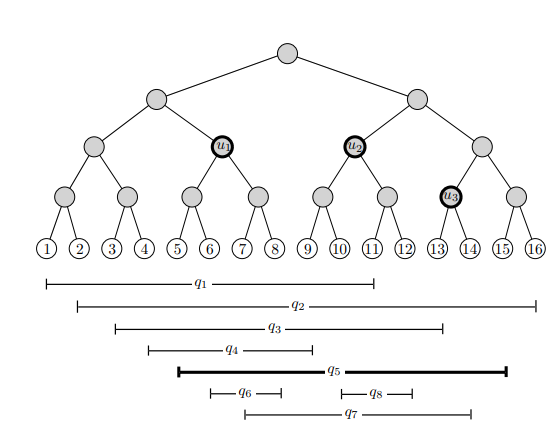
\includegraphics[scale=0.7]{thesis/figures/endpoint_tree.png}
\caption{An example of an endpoint tree with $I(u_3) = [13. 14)$, $I(u_2) = [9, 13)$ and $I(u_1) = [5, 9)$}
\end{figure}
\end{center}

\textbf{Applying Distributed Tracking.} We now reveal how nodes in the endpoint tree and their jurisdiction intervals coincide with RTS queries. Then, we will demonstrate how to effectively leverage Distributed Tracking algorithms to efficiently manage query maturation across the endpoint tree. First we require the following definition

\begin{definition}[Canoncial Node Set] For a given query $q\in Q^*$ with interval $R_q$ and endpoint tree $\mathcal{T}$ the \textit{Canonical node set} $U_q$ is the smallest $U_q\subseteq V(\mathcal{T})$ such that the jurisdiction intervals of $v\in U_q$ are pairwise disjoint and $R_q = \bigcup_{u\in U_q} I(u)$.
\end{definition}

For a given query $q$ with threshold $\tau_q$ and canonical node set $U_q$ we can consider a conceptual instance of distributed tracking with participants equal to $u_i\in U_q$, participant counters $c(u_i)$ as defined in the endpoint tree and coordinator threshold $\tau_q$. In this scenario, we view the query as the coordinator itself, whose mission is to capture the exact instant that 
\begin{equation}
    \tau_q = \sum_{u \in U_q} c(u) = W(q)
\end{equation}
We now execute an instance of \cref{alg:dist-tracking}, simulating each of its steps. We perform the element processing, and update each counter $c(u)$ in $\mathcal{T}$, these correspond to counter increments in \cref{alg:dist-tracking}. When condition $(3.1)$ is met via \cref{alg:dist-tracking}, this corresponds to query maturation in our range thresholding problem. 

As is emphasised in \cite{GAN16}, there is nothing \textit{distributed} in this configuration and all computation runs off of a single CPU. We simply leverage \cref{alg:dist-tracking} to efficiently identify the moment that an RTS query matures. To analyse the efficiency of the algorithm we will require the following lemmas:

\begin{lemma}
    For a given RTS query $q$ and endpoint tree $\mathcal{T}$, the canoncial node set $U_q$ can be determined in $O(\log m)$ time.
\end{lemma}
\begin{proof}
\end{proof}

\begin{lemma}
    For a given RTS query $q$ with canonical node set $U_q$ we have $|U_q| = O(\log m)$
\end{lemma}
\begin{proof}
\end{proof}

 As we have seen, each query $q\in Q^*$ defines an instance Distributed Tracking which we solve using \cref{alg:dist-tracking}. Recall from our description of \cref{alg:dist-tracking}, every node $u\in U_q$ maintains a counter $\Bar{c}_q(u)$ at the time of the last signal to the coordinator, $q$. The next signal from $u$ takes place 
\begin{equation}
    c(u) - \Bar{c}_q(u) = \lambda_q
\end{equation}
where $\lambda_q = \left\lfloor \frac{\tau_q}{2 |U|_q}\right\rfloor$ is the slack value described in \cref{alg:dist-tracking}. As part of the distributed tracking algorithm, the node $u$ needs to inspect condition (3.2) whenever $c(u)$ is incremented. By lemma 3.3 this implies $O(\log m)$ slack inspections per element processing. Theorem 2.5 gives the total messaging cost per query as $O(|U|_q\log \tau_q) = O(\log m\log\tau_q)$ by lemma 3.6.

\textbf{Organising Queries with Heaps.} The steps taken so far seem promising to result in a sub-quadratic algorithm, however let's pay close attention to the cost of inspecting the slack condition (3.2). For a given node $u\in V(\mathcal{T})$, let $Q(u)$ be the set set of queries that have $u$ in their canonical node set. Suppose that we have just incremented $c(u)$, if done naively, one would need to check condition $(3.2)$ for each $q\in Q(u)$. Clearly, this would require $O(|Q(u)|) = O(m)$ time, which coupled with $O(n\log m)$ element processing time for a stream of size $n$ would deprecate the performance of the algorithm to a quadratic $O(nm\log m)$.

Fortunately, with a few observations a we can leverage the Min-Heap described in \cref{sec:heap-data-structs} to avoid this. The idea is to inspect only \textit{one} slack condition in $Q(u)$, instead of all $|Q(u)|$. To see how one can do this, define for each $q$ the \textit{key}-value of 
\begin{equation}
    \sigma_q(u) := \lambda_q + \Bar{c}_q(u)
\end{equation}
where $\lambda_q, \Bar{c}_q$ correspond to values defined by \cref{alg:dist-tracking}. Intuitively $\sigma_q(u)$ represents the \textit{next} value of $c_q(u)$ for when the next signal from $u$ to coordinator $q$ should occur. The key observation is that, for $q_1, q_2 \in Q(u)$ with $\sigma_{q_{1}}(u) < \sigma_{q_{2}}(u)$ then $c_{q_1}(u) < c_{q_2}(u)$. That is, if we don't need to send a message for $q_1$, then we can immediately deduce that we do not need to send a messages for $q_2$. Using this key observation, we maintain a Min-Heap $\mathcal{H}(u)$ on $Q(u)$ for each $u\in V(\mathcal{T})$ and apply the following procedure whenever a counter is incremented.

\begin{algorithm}
\begin{algorithmic}[1]
\Procedure{SlackInspection}{$u$}
\State \text{Find the minimum $\sigma_q(u)$ in $\mathcal{H}(u)$}
\State \text{If $\sigma_q(u) < c(u)$, then we are done.}
\State \text{Otherwise, remove $\sigma_q(u)$ from       
             $\mathcal{H}(u)$. }
\Statex \text{\hspace{5mm} Instruct $u$ to send a signal to $q$ as per \cref{alg:dist-tracking}}
\Statex \text{\hspace{5mm} \textbf{return} SlackInspection$(u)$}
\Comment{Recursive call}
\EndProcedure
\end{algorithmic}
\end{algorithm}

We have the following result to analyse the 


\textbf{Analysis.} We have now motivated and explained each component of the DT algorithm. For the curious reader, we note that the algorithm is called \textit{DT} as a nod to it's use of \textit{Distributed Tracking}. We now prove correctness, and analyse the total complexity of the algorithm.

\begin{theorem}[Correctness] The Constrained DT algorithm solves the constrained RTS problem. That is, for each query $q$ the constrained DT algorithm correctly reports the instant that $W(q) = \tau_q$
\end{theorem}
\begin{proof}
    Each $q \in Q^*$ is mapped to an instance of Distributed Tracking which is then solved by \cref{alg:dist-tracking}. The correctness of reporting when $W(q) = \tau_q$ follows as a consequence of Theorem 2.5.
\end{proof}

\begin{theorem}[Time Complexity]
\end{theorem}


\subsection{Unconstrained RTS Case}
\clearpage

\def\chaptertitle{Dynamic Range Thresholding on Streams}

\lhead{\emph{\chaptertitle}}

\chapter{\chaptertitle}
\label{ch:drts}

For certain applications, one may be motivated to define a more general type of RTS query, in which the interval of interest \textit{evolves over time} with the data stream. Consider our first motivating example of a trader wanting to be alerted the moment some volume $\tau$ of Apple shares is traded between some price levels $[200, 205]$. In practice, the price levels of interest is likely to evolve over the day of the trading, or even widen with volatility. For example, a trader may wish to register a query of the form: \textit{notify me when $\tau$ volume of Apple shares are traded within 10\% of Apple's volume-weighted average price}. As one may recall, the volume-weighted average price (vwap) formula is given by 
$$\text{vwap} = \frac{\sum_{e} v(e) \cdot w(e)}{\sum_{e}w(e)}$$
which we clearly see evolves over the evolution of the data stream $\{e_i\}_{i=1}$.

In this chapter, we formally define this more general type of query, which we call a \textit{dynamic range threshold query} (DRTS query), then demonstrate that with minor adjustments, the DT algorithm discussed in \cref{ch:rts} is able to solve this more general type of query, though only when the number of \textit{distinct} DRTS queries is small (we will formally define exactly what we mean by \textit{distinct} later on). Finally, we introduce a novel approximation algorithm to handle a large number of distinct DRTS queries. 


\section{Problem Definition}
\label{sec:drts-problem-definition}

We define a Dynamic RTS (DRTS) query and then the dynamic range thresholding on streams problem.

\begin{definition}[Dynamic RTS query] A Dynamic RTS query is defined by a time-index triple $(R_t, \tau, f)$ where $\tau\in\mathbb{Z}$ is a \textit{threshold}, $f$ is a monotonically increasing  endpoint function and $R_t\subseteq \mathbb{R}^d$ is a time-indexed subset of the data space formed by axis-parallel rectangles. For $t =1,2,\dots$ the end points of each axis parallel rectangle $[a_t, b_t]$ are updated according to $[a_{t+1}, b_{t+1}]_i = [f(a_t), f(b_t)]_i$ for $i=1,\dots,d$ and $t=1,2,\dots$
\end{definition}

The dynamic range thresholding on streams problem is defined exactly as in \cref{sec:rts-definition}, though now with DRTS queries. That is, if a given query is issued after receiving $e_j$ for some $j\geq 1$ then for $t\geq j+1$ we define $S(q,t)$ to represent the elements $e_{j+1},e_{j+2},\dots,e_t$ that \textit{stab} $R_q$. That is, 
$$S(q, t) := \{e_i | j < i \leq t \text{ and } e_i \in R_q\}$$
Define
$$W(q, t) := \sum_{e\in S(q,t)}w(e)$$
Then the \textit{maturity time} of a query $q$ is the smallest $t$ such that $W(q,t)\geq \tau_q$. Our goal is to simultaneously support a set of $m$ DRTS queries and to correctly report the maturity time of a each query as well as the operations Register$(q)$: accept a new query at the current moment (after the arrival of $e_n$) and Terminate$(q)$: stop a given query $q$.

Some useful examples of DRTS queries are the following

\begin{example}[\textit{Equal Step DRTS}] Consider $m$ DRTS queries $(R_{qt}, \tau_q, f)$ on the one-dimensional data space  $\mathbb{R}$ with common endpoint function $f(x) = x + \Delta$ for a fixed constant $\Delta\in\mathbb{R}$. Conceptually, such an endpoint function moves the each query to the left or right (depending on the sign of $\Delta$) by a factor of $\Delta$ after each time step.
\end{example}

\begin{example}[\textit{Equal Expansion DRTS}] Consider $m$ DRTS queries $(R_{qt}, \tau_q, f)$ on the one-dimensional data space  $\mathbb{R}$ with common endpoint function $f(x) = \Delta x$  for a fixed constant $\Delta\in\mathbb{R}$. Conceptually, such an endpoint function expands the length of each query by an order of $\Delta$ on each time step.
\end{example}
    
We note that definition 4.1 leaves few restrictions on the possible choices for the endpoint function $f$, only that it be monotonically increasing so that the interval remains well defined after each time step. One could therefore supply a multivariate function $f(x,t)$ such as $f(x, t) = x + \Delta_t$ for some sequence $\{\Delta_t: t\geq1\}$. Thus, proposed solutions to the DTS problem must be able to solve these types of queries also. 


\newpage
\section{DT Algorithm For DRTS Queries}
\label{sec:drts-dt-algorithm}

The goal of this section is to demonstrate that with minor enhancements, the DT algorithm can solve certain DRTS queries. Moreover, we then characterise exactly what DRTS queries our new algorithm is able to solve. First we need to consider two versions of the Dynamic Range Thresholding on Streams problem: 

\begin{definition}[Distinct \& Non-Distinct Dynamic RTS]
    Conisder $m$ DRTS queries $(R_{t}^q, \tau_q, f_q)$ if all queries share the same endpoint function, that is for all $1\leq i\leq  j\leq m$ we have $f_i = f_j$ then we classify this instance as the \textit{Non-Distinct} DRTS problem. In the case where any of the two queries have different endpoint functions, we call this an instance of the \textit{Distinct DRTS} problem.
\end{definition}

Clearly, the non-distinct DRTS problem offers us a simpler problem instance from which we can first design our enhanced algorithm. We then apply some standard techniques to extend to the distinct case. 

\subsection{Non-Distinct DRTS}
\label{ssec:non-distinct-rts}

We consider the scenario in which all 
% \input{chapters/03-semantics.tex}
% \input{chapters/04-types.tex}
% \input{chapters/05-resources.tex}
% \input{chapters/06-lpvm-conversion.tex}
% \input{chapters/07-lpvm-optimisations.tex}
% \input{chapters/08-llvm-conversion.tex}
% \input{chapters/09-experiments.tex}
% \input{chapters/10-conclusion.tex}

\addtocontents{toc}{\vspace{2em}}

%TC:ignore
\appendix
% \clearpage

\def\chaptertitle{Evaluation Data}

\lhead{\emph{\chaptertitle}}

\chapter{\chaptertitle}
\label{apx:data}

\newcommand{\timetable}[4]{
  \footnotesize
  \def\arraystretch{.7}
  \begin{longtable}[ht]{rl*{8}{S[tight-spacing=true, table-format=1.3, round-mode=places, round-precision=3]}}
    \caption{#3}
    \label{#4} \\
    \toprule Program & #1 & \multicolumn{8}{l}{Time (\si{\second})} \\ \midrule\endfirsthead
    \caption[]{#3} \\
    \toprule Program & #1 & \multicolumn{8}{l}{Time (\si{\second})} \\ \midrule\endhead
    \bottomrule\endfoot
    \csvreader[
      late after line=\\ \ifodd\thecsvrow\midrule\fi,
      head to column names, head to column names prefix=the
    ]{#2}{}{
      \ifodd\thecsvrow\theprog\fi & \theclass & \thetimeA & \thetimeB & \thetimeC & \thetimeD & \thetimeE & \thetimeF & \thetimeG & \thetimeH \\
      & & \thetimeI & \thetimeJ & \thetimeK & \thetimeL & \thetimeM & \thetimeN & \thetimeO & \thetimeP \\
      & & \thetimeQ & \thetimeR & \thetimeS & \thetimeT & \thetimeU & \thetimeV & \thetimeW & \thetimeX \\
      & & \thetimeY & \thetimeZ & \thetimeAA & \thetimeAB & \thetimeAC & \thetimeAD 
    }
  \end{longtable}
}
    
\timetable{Order}{\datapath/time-order-clean.csv}
  {Runtime of first-order and higher-order program implementations.}
  {tab:order}

\timetable{Resource}{\datapath/time-resources-clean.csv}
  {Runtime of first-order programs with globalised and parameterised resources.}
  {tab:resources}

% \input{appendices/programs.tex}
%TC:endignore

\addtocontents{toc}{\vspace{2em}}
\backmatter

\lhead{\emph{Bibliography}}
\bibliographystyle{unsrtnat}
\bibliography{thesis}
\label{bibliography}

\end{document}
